\section{Grundlagen Distributed Ledger Technology}
In diesem Grundlagen Kapitel soll ein Verständnis für die unterschiedlichen Begriffe und Verfahren der Blockchain Technologie etabliert werden. Beginnend mit einer allgemeinen Definition des Begriffs Blockchain, werden die verschiedenen Arten von \ac{dlt} im Detail betrachtet und definiert. Eine Abgrenzung zu Kryptowährungen soll zeigen, dass Blockchain nicht gleich Kryptowährungen bedeutet. In Kapitel 2.4 wird der technologische Hintergrund erörtert und abschließend soll eine Auflistung der vorhandenen \ac{dlt} die aktuelle Herstellerlandschaft zeigen.

\subsection{Definition}
Unter dem Begriff Blockchain wird eine Technologie verstanden, die eine erweiterbare Liste von Datensätzen bildet. Jeder Eintrag in dieser Liste wird Block genannt und ist durch kryptographische Methoden untereinander verkettet. Als Inhalt besitzt jeder Block einen kryptographischen Hashwert des vorhergehenden Blocks, sowie einen Zeitstempel und die eigentlichen Daten.\cite[Vgl.]{narayanan2016bitcoin} (Abbildung \ref{fig:simple-blockchain-schema})
\begin{figure}[h!]
	\centering
	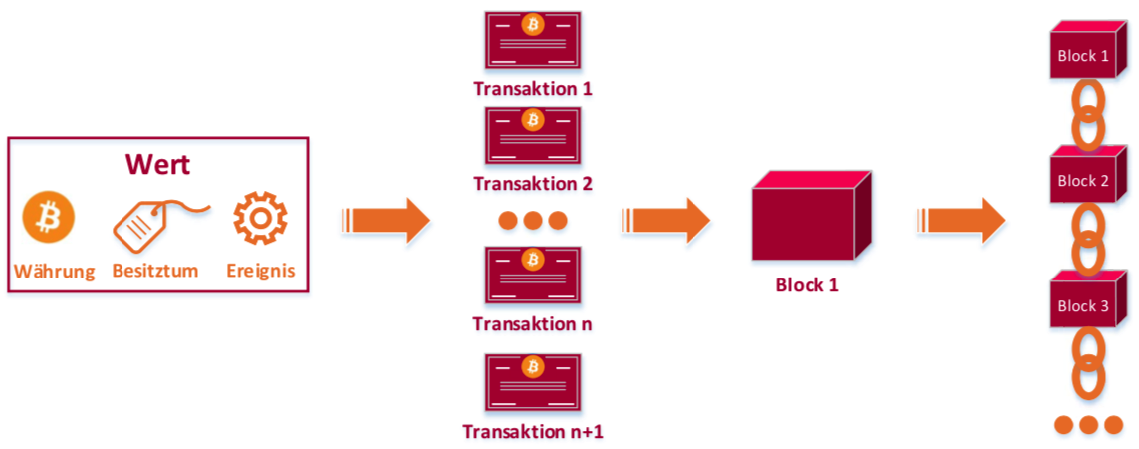
\includegraphics[width=1.0\linewidth]{pictures/simple-blockchain-schema}
	\caption[Vereinfachte Darstellung einer Blockchain]{Vereinfachte Darstellung einer Blockchain\cite{Gayvoronskaya2017}}
	\label{fig:simple-blockchain-schema}
\end{figure}

Technisch ist eine Blockchain also eine Art dezentrale Datenbank. Das Netzwerk aus Teilnehmern der Blockchain entscheidet im Konsens welcher Block (Datensatz) valide ist und der Gesamtmenge an Blöcken (Datenbank) angehangen wird. Zur Konsensbildung werden spezielle Algorithmen verwendet, um einen sog. byzantinischen Fehler zu verhindern. Durch die Vielzahl der Teilnehmer kann das mögliche Fehlermodell bei der Konsensbildung sehr komplex und schwer zu erfassen sein. Darauf beziehen sich byzantinische Fehler und die vorhandenen Lösungsansätze.

Der Oberbegriff \acf{dlt} wird in diesem Kontext gleichermaßen Synonym verwendet. Jedoch muss nicht zwingend jedes \glqq Distributed Ledger\grqq{} eine Blockchain als technische Grundlage verwenden. Viele unterschiedliche Ansätze werden aktuell in der Forschung und freien Marktwirtschaft erprobt und auf ihre Eigenschaften hin untersucht.\cite[Vgl.]{Mitschele2018}

Das hohe Maß an Sicherheit, welches mit dem Begriff Blockchain assoziert wird, wird durch die Signierung der Blöcke und Transaktionen mit dem Public-Key-Verfahren garantiert. Auf dieses kryptographische Verfahren wird in Kapitel \ref{tec_bkgrnd_sec} näher eingegangen. In klassischen verteilten Datenbanken oder Systemen hat eine zentrale Organisation oder Kontrolleinheit als einzige die Möglichkeit den Datenbestand in einem konsistenten Zustand zu halten. Viel mehr ist diese zentrale Organisation der Vertrauensgeber des Systems - ohne Schutz vor Missbrauch. Um einem Missbrauch vorzubeugen sind \ac{dlt} dezentral organisiert. Dies bedeutet das es keine zentrale Einheit benötigt um Vertrauen über die Korrektheit der Transaktionen herzustellen.\cite[Vgl.]{Welzel2017} Abbildung \ref{fig:change-in-transaction-model-blockchain} veranschaulicht die Veränderung des Transaktionsmodells durch \ac{dlt}.
\begin{figure}[h!]
	\centering
    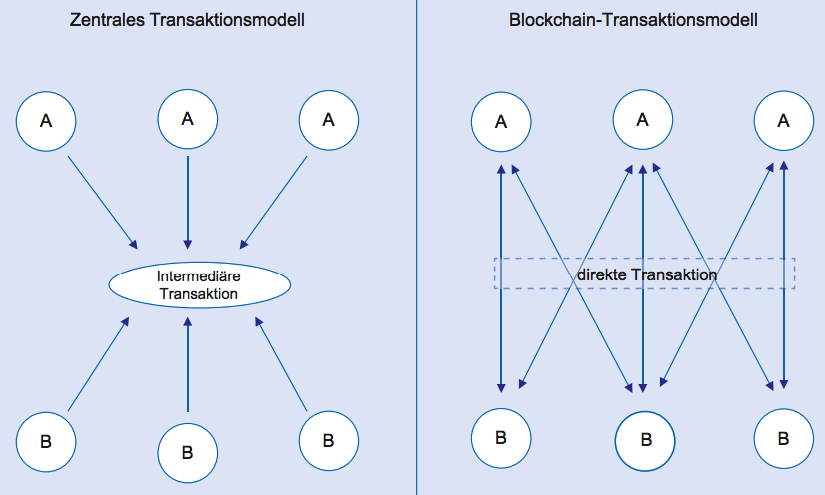
\includegraphics[width=0.76\linewidth]{pictures/change-in-transaction-model-blockchain}
	\caption[Veränderung des Transaktionsmodells durch die Blockchain]{Veränderung des Transaktionsmodells durch die Blockchain\cite{Kastrati2016}}
	\label{fig:change-in-transaction-model-blockchain}
\end{figure}

Die älteste sich noch in Betrieb befindliche \ac{dlt} ist die Blockchain der Kryptowährung \ac{btc}.

\subsection{Technologischer Hintergrund}
Der technologische Hintergrund bei DLT hat verschiedene Fundamente. Sicherheit wird durch Kryptographie hergestellt. Insbesondere werden digitale Signaturen verwendet um Transaktionen fälschungssicher zu erzeugen und über das Netzwerk zu verteilen. Unterschiedlichste Konsensalgorithmen kommen zum Einsatz um ein Konsistenten Zustand zu garantieren. Das Netzwerk selbst ist ein Peer-to-Peer Netzwerk. Ein Netzwerk, dass auf dem normalen Internet aufsetzt und operiert. Außerdem bietet DLT die möglichkeit des verteilten Computing durch sog. Smart Contracts die im Netzwerk gespeichert und von diesem auch ausgeführt werden.

\subsubsection{Sicherheit} \label{tec_bkgrnd_sec}
Sicherheit ist eines der Hauptmerkmale einer DLT. Zum einen müssen die Konten bzw. Accounts der Teilnehmer ausreichend geschützt sein vor Missbrauch oder Diebstahl. Zum anderen müssen Transaktionen zwischen Teilnehmern so gesichert sein, dass alle Teilnehmer im Netzwerk die authentizität prüfen können ohne die Parteien der Transaktion direkt kennen zu müssen. Diese Anforderungen werden durch kryptographische Methoden sichergestellt die nachfolgend näher ausgeführt werden.

\paragraph{Public-Key Authorization}
\begin{figure}[h!]
	\centering
	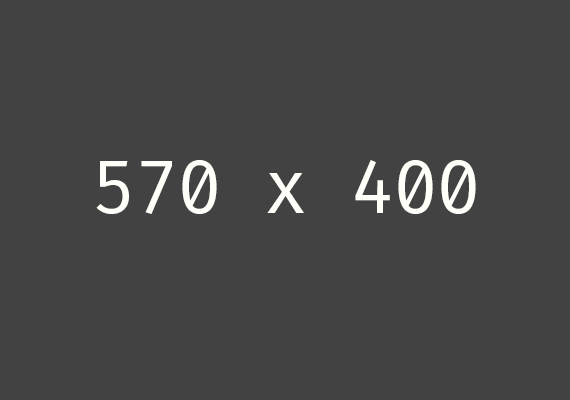
\includegraphics[width=1.0\linewidth]{pictures/placeholder_half_page}
	\caption[Placeholder Half Page]{Placeholder Half Page}
	\label{fig:placeholder_half_page}
\end{figure}
- Verwendete Algorithmen
- Public Keys
- Private Keys
- Multi-Sig

\paragraph{Hashing Algorithmus}
- Algorithmen
- Allgemeine Erklärung Hash Funktion

\subsubsection{Konsensalgorithmen}
byzantinische Fehler als Ursprung des Konsensproblems. Verschiedene Ansätze vorhanden um dieses Problem zu lösen. Darunter Proof-of-Work (Bitcoin), Proof-of-Stake (Ethereum nach Caspar), Delegated Proof-of-Stake (EOS).


\paragraph{Proof-of-Work}
\begin{figure}[h!]
	\centering
	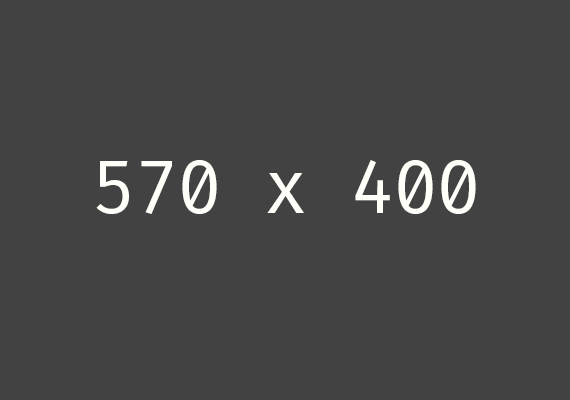
\includegraphics[width=1.0\linewidth]{pictures/placeholder_half_page}
	\caption[Placeholder Half Page]{Placeholder Half Page}
	\label{fig:placeholder_half_page}
\end{figure}


\paragraph{Proof-of-Stake}
\begin{figure}[h!]
	\centering
	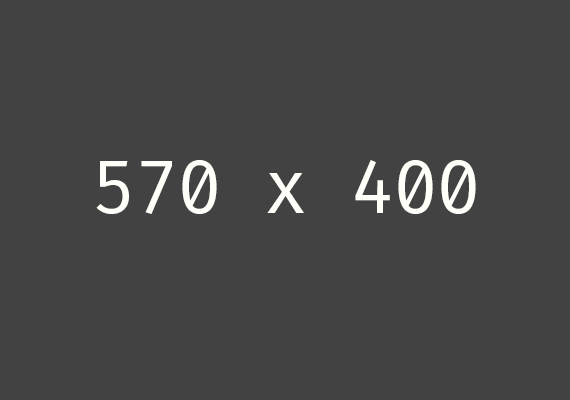
\includegraphics[width=1.0\linewidth]{pictures/placeholder_half_page}
	\caption[Placeholder Half Page]{Placeholder Half Page}
	\label{fig:placeholder_half_page}
\end{figure}


\paragraph{Delegated Proof-of-Stake}


\subsubsection{Netzwerke}
\begin{figure}[h!]
	\centering
	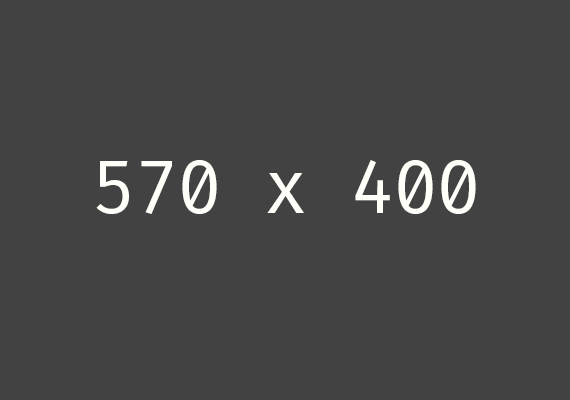
\includegraphics[width=1.0\linewidth]{pictures/placeholder_half_page}
	\caption[Placeholder Half Page]{Placeholder Half Page}
	\label{fig:placeholder_half_page}
\end{figure}
- Herkunft
- Technologie

\paragraph{Peer-to-peer Netzwerke}

\paragraph{Business Netzwerke}

\subsubsection{Distributed Computing}


\subsection{Ausprägungen von \acl{dlt}}
Neben dem Blockchain Ansatz existieren noch weitere Ideen eines \ac{dlt}. Die aktuell am weitesten fortgeschrittenen Projekte sind das Ethereum Projekt, der sog. \glqq Tangle\grqq{} von der Iota Foundation und die \glqq HashGraph\grqq{} genannte Technologie von Leemon Baird.\cite{Baird2016} Außerdem lassen sich \ac{dlt} in öffentlich-, privat- und konsortium Geführte Lösungen kategorisieren. Einige Ansätze lassen sich zu mehr als einer Kategorie zuordnen. Dies wird in den folgenden Unterkapiteln näher untersucht.

\subsubsection{Blockchain}
\begin{figure}[h!]
	\centering
	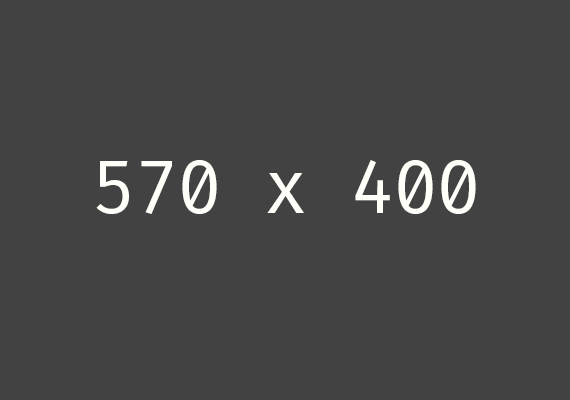
\includegraphics[width=1.0\linewidth]{pictures/placeholder_half_page}
	\caption[Placeholder Half Page]{Placeholder Half Page}
	\label{fig:placeholder_half_page}
\end{figure}
- Herkunft
- Technologie

\subsubsection{Tangle}
- Herkunft
- Technologie

\subsubsection{Hash Graph}
\begin{figure}[h!]
	\centering
	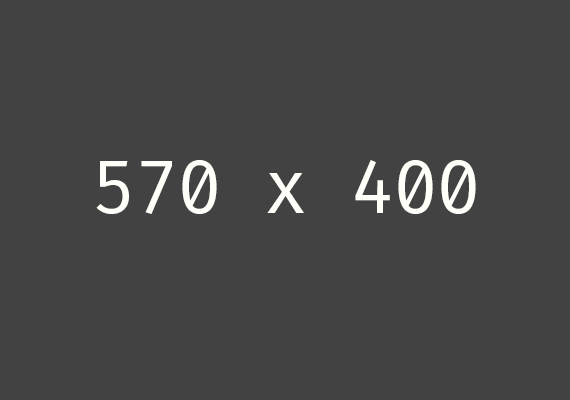
\includegraphics[width=1.0\linewidth]{pictures/placeholder_half_page}
	\caption[Placeholder Half Page]{Placeholder Half Page}
	\label{fig:placeholder_half_page}
\end{figure}
- Herkunft
- Technologie

\subsubsection{Public}
- Vorteile
- Nachteile

\subsubsection{Private}
- Vorteile
- Nachteile

\subsubsection{Consortium}
\begin{figure}[h!]
	\centering
	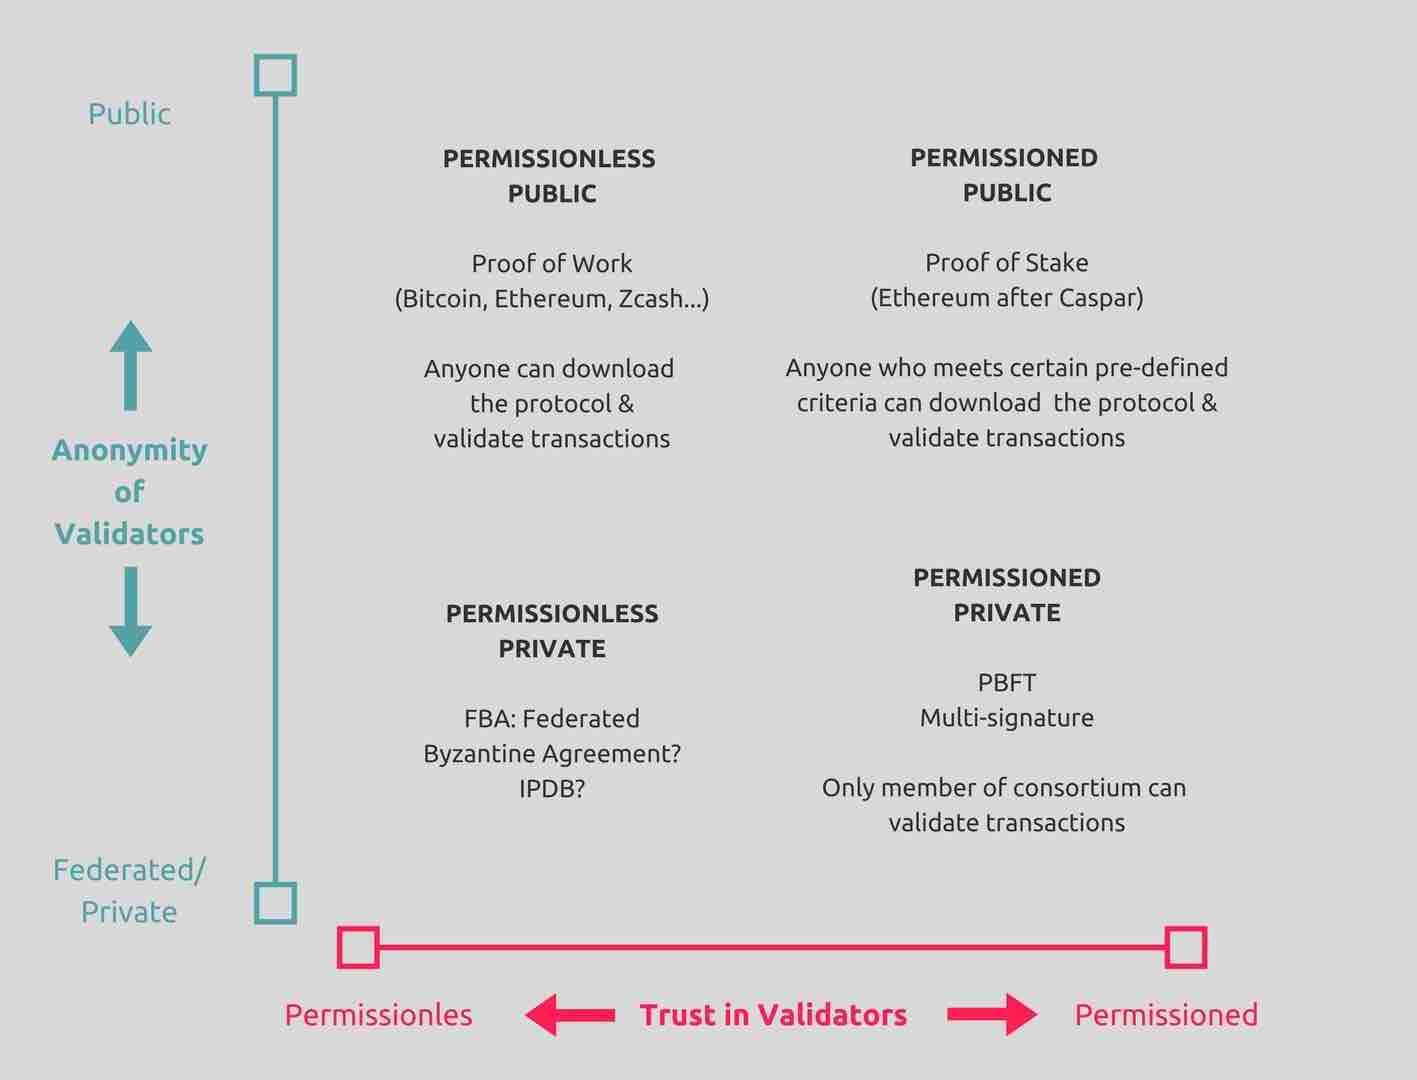
\includegraphics[width=1.0\linewidth]{pictures/dlt-type-matrix}
	\caption[DLT Type Matrix]{DLT Type Matrix}
	\label{fig:dlt-type-matrix}
\end{figure}
- Vorteile
- Nachteile

\subsection{Abgrenzung Kryptowährungen}
Blockchain ist nicht gleich Bitcoin. Mit dem Bitcoin Protokoll wurde die erste Blockchain verwendet. Erfinder ist bis heute unbekannt. Auszüge Whitepaper

\subsection{Vorhandene Distributed Ledger}


\subsubsection{Bitcoin}


\subsubsection{Ethereum}


\subsubsection{IOTA}


\subsubsection{Ripple}


\subsubsection{IBM Bluemix}


\subsubsection{Microsoft Azure}


\subsubsection{Hyperledger Fabric}


\newpage
